\section{Related Work}

\begin{frame}{Related Work}
       \tableofcontents[sectionstyle=show/hide, hideothersubsections]
    \begin{center}
    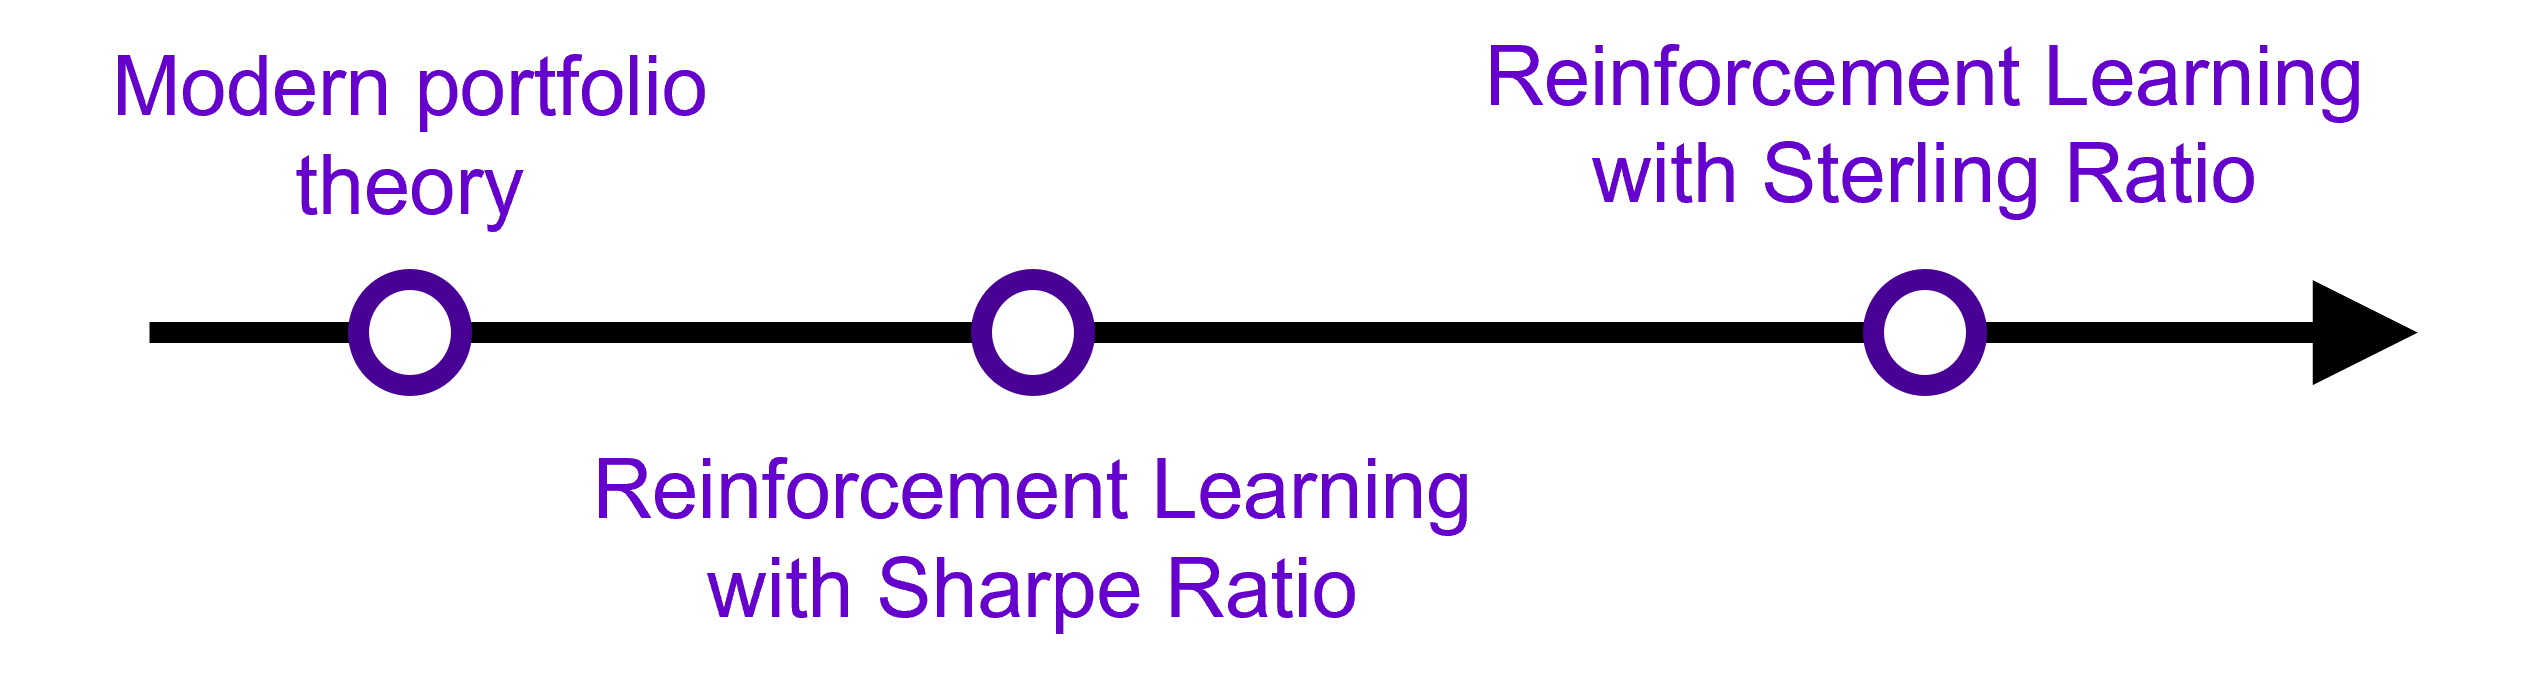
\includegraphics[width=10cm]{images/related.png}
    \end{center}
\end{frame}

\subsection{Modern Portfolio Theory}
\begin{frame}
\frametitle{Modern Portfolio Theory (MPT)}
\begin{columns}
\begin{column}{0.55\textwidth}
MPT produces portfolios with maximum expected return from given risk (variance) or vice versa base on the forecasts of future performance (expected return and variance)
\end{column}
\begin{column}{0.45\textwidth}
\begin{center}
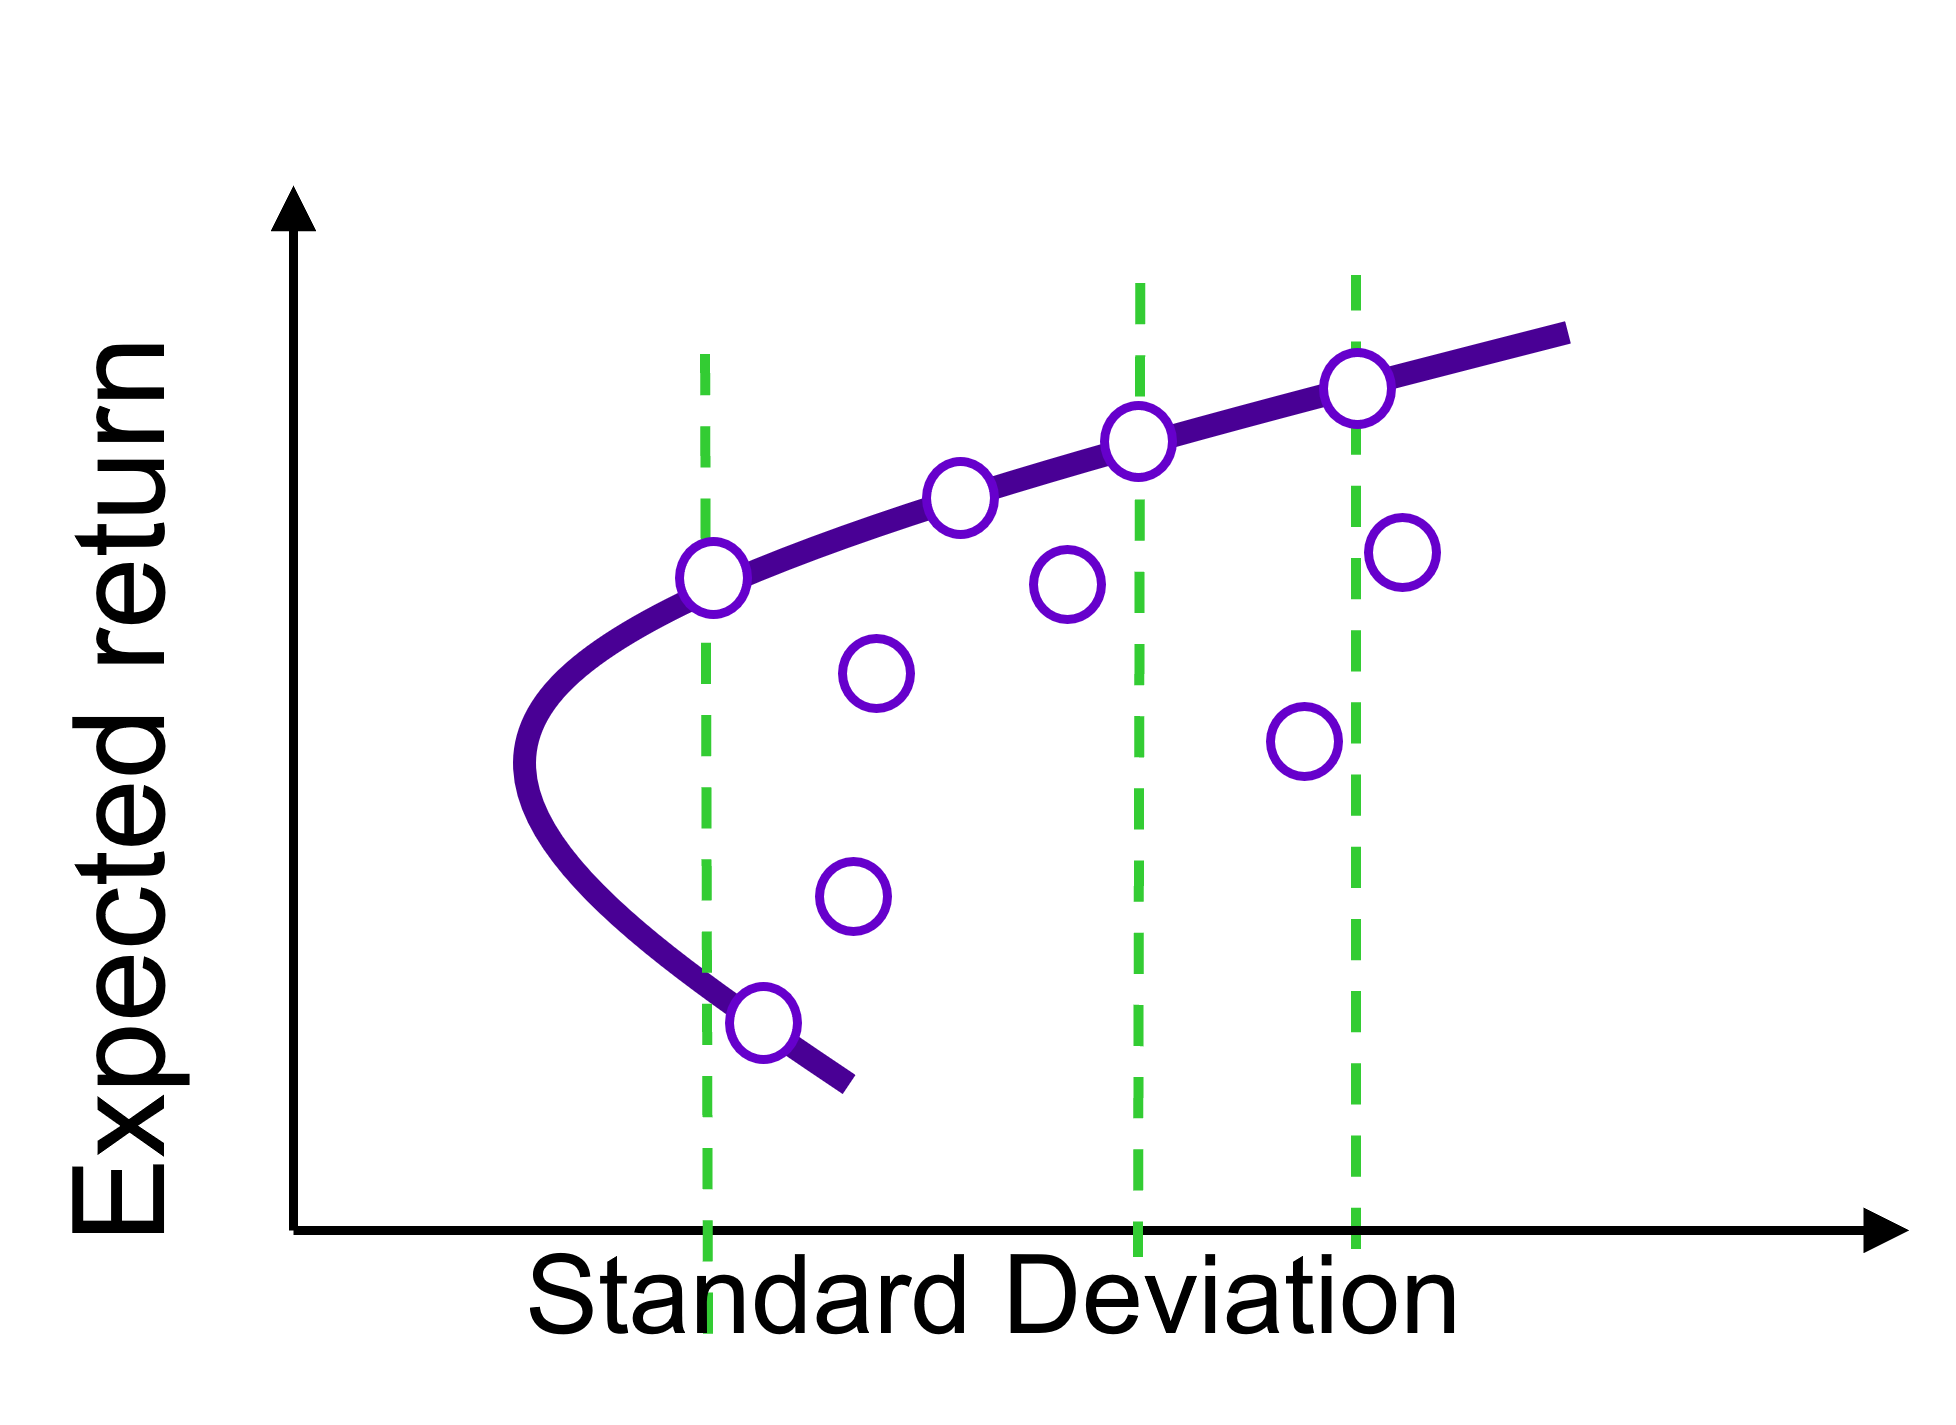
\includegraphics[width=4.8cm]{images/mpt_risk.png}
\end{center}
\end{column}
\end{columns}
\end{frame}


\subsection{Reinforcement Learning with Sharpe Ratio}
\begin{frame}{Reinforcement Learning with Sharpe Ratio}
John Moody's trading system used reinforcement learning to construct the optimal portfolio and used Sharpe Ratio as objective function.

\begin{block}{Sharpe Ratio}
\[ SR = \frac{E(R_a - R_b)}{\sigma_a}\]
\(R_a\): the return of the assert
\\
\(R_b\): the risk-free return
\\
\(E(R_a - R_b)\): the expected excess return of the assert
\\
\(\sigma_a\): standard deviation of the excess return.
\end{block}
\end{frame}



\begin{frame}{The differential Sharpe ratio}
Online learning systems required influence on Sharpe ratio, an incremental Sharpe ratio, or differential Sharpe ratio \(D_t\).
\begin{block}{Differential Sharpe Ratio}

\[
\cfrac{d D_t}{d R_t} = 
\cfrac{B_{t-1}-A_{t-1} R_t}{(B_{t-1}-A_{t-1}^2)^\frac{3}{2}}
\]
where
A and B is the first and second moments of the returns' distributions
\[ A_n = \cfrac{1}{n}\sum_{i=1}^nR_i\quad
B_n = \cfrac{1}{n}\sum_{i=1}^nR_i^2
\]
\end{block}
\end{frame}



\subsection{Reinforcement Learning with Sterling Ratio}
\begin{frame}{Reinforcement Learning with Sterling Ratio}
\begin{block}{Problem}
Sharpe ratio is criticized for adjustment done based on variance rather than downside risk, penalty upon large positive returns.
\end{block}
\begin{block}{Solution}
Use Sterling Ratio as objective function.
\[
Sterling Ratio=\frac{Annualized Average Return}{Maximum Drawdown}
\]
\end{block}

\end{frame}

\begin{frame}{Alternatives to Maximum Drawdown and  Sterling Ratio}
Maximum Drawdown is cumbersome to minimize.
Moody used DD to replace , the square root of the average of the
square of the negative returns, defined as
\[
DD_T = \sqrt{\cfrac{1}{T}\sum_{t=0}^{T}{min\{R_T,0\}^2}}
\]
And replace Sterling Ratio with downside deviation ratio (DDR)
\[
DDR_T = \frac{Average(R_T)}{DD_T}
\]
\end{frame}


\begin{frame}{Differential form}
The reward function will use the differential form of the utility function \(D_t\).

\begin{block}{Differential Form}

\[
D_t = 
\begin{cases}
    \cfrac{R_{t-1} -\frac{1}{2}A_{t-1}}{DD_{t-1}},&\text{if  }R_t > 0\\
    \cfrac{DD_{t-1}^2 (R_{t-1}-\frac{1}{2}A_{t-1})  -\frac{1}{2}A_{t-1} R_t^2}{DD_{t-1}^3},&\text{if  }R_t \leq 0
\end{cases}
\]
\end{block}
Unlike utility functions that use variance as the risk-adjusted factor, this formula indicates no penalty for large positive returns. 

\end{frame}


\subsection{Comparison}
\begin{frame}{Comparison}
    \centering
    \begin{tabular}{|| c|c|c|| }
    \hline \hline
    Portfolio Management System & Adjustable risk preferences & Alternative input sources \\     \hline \hline
    MPT & \color{blue}{Yes} & No \\  \hline
    RL with Sharpe/Sterling ratio& No & \color{blue}{Yes}  \\  \hline
    Proposed System & \color{blue}{Yes} & \color{blue}{Yes} \\   \hline \hline
    \end{tabular}

\end{frame}